\section{Introduction}
\label{sec:Introduction}

Niobium cavities have been extensively studied and treatments have been developed to optimize the accelerating gradient and quality factor~\cite{10.1063/1.4866013, 10.1063/1.4960801, 10.1063/5.0059464, 10.1063/5.0063379}. The performance of niobium SRF cavities is limited by the material properties of niobium (Nb). A promising alternative to Nb is Nb\textsubscript{3}Sn. There exists a large body of research on creating high performance Nb\textsubscript{3}Sn superconducting radiofrequency (SRF) cavities\cite{10.1063/1.4913617, 10.1063/1.4913247}. Desirable superconducting properties, such as higher superconducting transition temperature (T\textsubscript{c}) and a higher superheating magnetic field (H\textsubscript{sh})\cite{liarte2017theoretical, catelani2008temperature, lin2012effect, kubo2020superfluid}, make Nb\textsubscript{3}Sn an attractive material for SRF applications. The material properties of Nb\textsubscript{3}Sn, however, make it difficult to work with. 

The brittleness of Nb\textsubscript{3}Sn introduces new challenges to the cavity manufacturing process. Nb\textsubscript{3}Sn must be deposited as a thin film on a bulk cavity substrate\cite{posen2017nb3sn, pudasaini2019growth, porter2018update}. Because of the thin and brittle film, Nb\textsubscript{3}Sn cavities are highly susceptible to mechanical stress. Nb\textsubscript{3}Sn cavity performance is known to permanently degrade when stresses are applied to the cavity\cite{eremeev2023preservation, eremeev:srf2019-mop015}. This degradation is assumed to be caused by cracks in the brittle Nb\textsubscript{3}Sn film caused by deformation of a cavity during processing such as tuning or assembly. Cavities that suffer from degradation are typically stripped and recoated with a new Nb\textsubscript{3}Sn film, which is a time-consuming and expensive process.

In this current study we explore a new procedure to heal Nb\textsubscript{3}Sn cavities whose performance has been degraded by deformation. This procedure utilizes a short Nb\textsubscript{3}Sn recoating to attempt to heal cracks that have formed in the cavity without the need to remove the original film. This procedure was developed to restore the performance of a Nb\textsubscript{3}Sn cavity which has undergone centrifugal barrel polishing\cite{viklund2024improving}. The performance decrease measured on a polished cavity is like the above mentioned case of deformation-induced degradation. When employing this recoating procedure to a degraded cavity, we can recover a large portion of the performance with a simple furnace treatment. This discovery provides a valuable method for recovering degraded cavities without lengthy reprocessing which avoid subsequent thinning and frequency shifts.


\section{Experiment}
\label{sec:Experiment}

This study is performed on a Nb\textsubscript{3}Sn, \qty{1.3}{\giga\hertz} cavity coated using a high-temperature nucleation step to create a Nb\textsubscript{3}Sn film with low surface roughness. An in-depth analysis of this cavity coating and the initial performance of the cavity can be found in reference~\cite{posen2021advances}. 

After initial testing, the cavity was transported to Cornell, after which performance decreased. The cavity was then returned back to FNAL for additional testing, which confirmed the performance degradation. We suggest that the degradation was caused by stresses applied to the cavity during transport, which led to the formation of cracks. This type of performance degradation has previously been observed during assembly of Nb\textsubscript{3}Sn cavities~\cite{eremeev2023preservation}, and when tuning Nb\textsubscript{3}Sn cavities at room temperature~\cite{eremeev:srf2019-mop015}. In these cases, stresses applied to the cavity were suggested to be the main cause of the degradation. Cracks may also form in Nb\textsubscript{3}Sn cavities as a result of stress concentrators such as foreign particles or impurities located in the Nb-Nb\textsubscript{3}Sn inferface. Another possible source of performance degradation is elastic deformation of the Nb\textsubscript{3}Sn film caused by thermal contration of the cavity during cooldown. This is, however, unlikely in this case since the thermal expansion coeficcient of Nb and Nb\textsubscript{3}Sn does not differ enough to cause degradation, and Nb\textsubscript{3}Sn cavities have shown no signs of degradation due to thermal cycling.

To heal the cracks causing the performance degradation, we apply a recoating procedure. During this recoating procedure, the cavity was heated to \qty{1000}{\degreeCelsius} and exposed to Sn vapor for \qty{1}{\hour}. Sn vapor was provided by \qty{0.85}{\gram} of Sn heated to \qty{1250}{\degreeCelsius}. The reasoning behind these parameters is that only a small amount of Sn is necessary to fill the microscopic cracks in the film. Applying too much Sn causes the film to become too thick and negatively impacts the surface roughness of the film. During the coating process only a small fraction of the Sn evaporated leaving behind a large amount of the initial Sn still in the crucible. 

The cavity performance was tested using a vertical testing stand (VTS). The cavity was tested before degradation, after degradation, and after recoating at \qty{4}{\kelvin} and at \qty{2}{\kelvin}. The cavity was cooled down below its superconduting transition temperature at \qty{16}{\kelvin} at a slow cooling rate of \qty{0.1}{\kelvin\per\minute} to minimize trapped flux. Between each test the cavity was brought up to a temperature above its superconducting transition temperature and cooled back down using the slow cooling rate to eliminate any trapped flux caused by cavity quenching. Temperature mapping was performed during the VTS test at \qty{2}{\kelvin}.

\section{Results}
\label{sec:Results}

\begin{figure}[h]%
    \centering%
    \includegraphics[width=1.0\columnwidth]{./figures/VTS.png}%
    \caption{The quality factor, indicated by dots, and X-ray emissions, indicated by x, versus the accelerating gradient of the cavity after the initial coating (A), after the degradation (B), and after the recoating (C). The quality factor and accelerating gradient of the T-maps in figure~{\protect\ref{fig:TMAP}} are indicated by a red star.}%
    \label{fig:VTS}%
\end{figure}

\begin{figure}[h]%
    \centering%
    \includegraphics{./figures/TMAP.png}%
    \caption{Temperature maps of a cavity's surface prior to quench as measured before (top) and after (bottom) the recoating is applied. The temperature maps are measured at \qty{2}{\kelvin}. The sensor number corresponds to different regions of the cavity. Sensor 1 and 16 are near the top and bottom iris while sensor 8 is on the equator. The quality factor and accelerating gradient of the cavity during the measurement is shown be the red star in figure~{\protect\ref{fig:VTS}}. The temperature of the hot spot near the equator of the recoated cavity exceeds the maximum value of the color bar and achieves a maximum value at \qty{3}{\kelvin}}%
    \label{fig:TMAP}%
\end{figure}

After initially coating the cavity it achieves a peak accelerating field of \qty{24}{\mega\volt\per\meter} and a maximum Q of \num{2e10} at \qty{4}{\kelvin}. The peak accelerating gradient after degradation is \qty{8}{\mega\volt\per\meter} and a maximum Q of \num{2e10} at \qty{4}{\kelvin}. The cavity displays a decrease in the quality factor at around \qty{6}{\mega\volt\per\meter} before a quench. A similar decrease in the quality factor is observed for other cavities affected by performance degradation\cite{eremeev2023preservation,eremeev:srf2019-mop015} and in Nb\textsubscript{3}Sn cavities treated with centrifugal barrel polishing\cite{viklund2024improving}. Temperature mapping is displayed in figure~\ref{fig:TMAP} and is utilized to locate the quench source responsible for the performance degradation. A single hot spot on the equator of the cavity is present. Visual inspection of the cavity did not display visible defects near the quench location.

After the recoating procedure is applied the cavity's performance increases. The cavity experiences an initial quench at \qty{16}{\mega\volt\per\meter} resulting in trapped flux which decreases the quality factor. The cavity is still able to reach a peak accelerating gradient of \qty{19}{\mega\volt\per\meter}. At \qty{2}{\kelvin} the cavity does not quench until reaching the maximum gradient of \qty{19}{\mega\volt\per\meter}. The quality factor after recoating is \num{2e10} at \qty{4}{\kelvin} and the Q slope seen in the degraded cavity is not present. Temperature mapping of the cavity after recoating demonstrates that the initial hot spot is healed with no detectable heating from that area. This indicates that the defect causing the performance degradation is repaired by recoating. At higher gradients another small hotspot appears in a new location close to the equator, and there is also a larger hot spot closer to the iris, which appears just before the cavity quench. We also see a spike in the x-ray emissions from the cavity just before the final quench at \qty{4}{\kelvin}. Although we are not certain what the cause of this spike is, it does not seem to be caused by the cracks nor the recoating. This particular cavity has shown x-ray emissions in the past even before the degradation and recoating occured.

\section{Evidence of Crack Healing Mechanism in Nb\textsubscript{3}Sn}

To study the healing mechanism of the recoating procedure, we purposefully introduce cracks into Nb\textsubscript{3}Sn coated Nb wires. \qty{3}{\milli\meter} diameter low RRR Nb wires were coated with Nb\textsubscript{3}Sn using Sn vapor diffusion. Before the coating, the Nb wires are electropolished and anodized in the same way as Nb\textsubscript{3}Sn cavities. Cracks are created by elongating the wires using an Instron tensile testing machine. We then cut the wires into two pieces and treat one half of the wires with the same recoating recipe shown in section~\ref{sec:Experiment}. The cracks are analyzed before and after recoating using scanning electron microscopy (SEM) and energy dispersive x-ray spectroscopy (EDS). 

The elongation of the wires causes intragranular cracks to form perpendicular to the direction of applied stress as shown in figure~\ref{fig:SEM}. A cross section of the sample, as seen in figure~\ref{fig:EDS}, show that the cracks penetrate all the way through the Nb\textsubscript{3}Sn film and stop at the Nb substrate giving the crack a rectangular profile with sharp \qty{90}{\degree} edges. These cracks can be considered an extreme example of the cracks we expect to see in Nb\textsubscript{3}Sn cavities since the wires are heavily deformed in the plastic regime. In contrast, cracks formed in Nb\textsubscript{3}Sn cavities are formed during elastic deformation of the niobium substrate or only slight plastic deformation which does not significantly impact the geometry of the cavity. Therefore, we expect cracks in degraded cavities to be smaller than what is seen in this study.

After the recoating, the cracks appear to be partially healed. Figure~\ref{fig:SEM} shows some of the cracks being partially filled in with new material creating a discontinuous crack. Additionally, the sharp edges of the untreated cracks have been smoothed out due to deposition of new material. The cross section of the sample in figure~\ref{fig:EDS} shows that new Nb\textsubscript{3}Sn is created both within the crack and at the exposed Nb substrate at the base of the crack. Since the cracks produced by elongating the wires are larger than what we expect in Nb\textsubscript{3}Sn cavities, it is likely that the cracks formed in cavities can be completely healed using this recoating recipe. It may also be possible to increase the recoating duration or temperature to allow larger cracks to heal completely as well.

\begin{figure}
    
    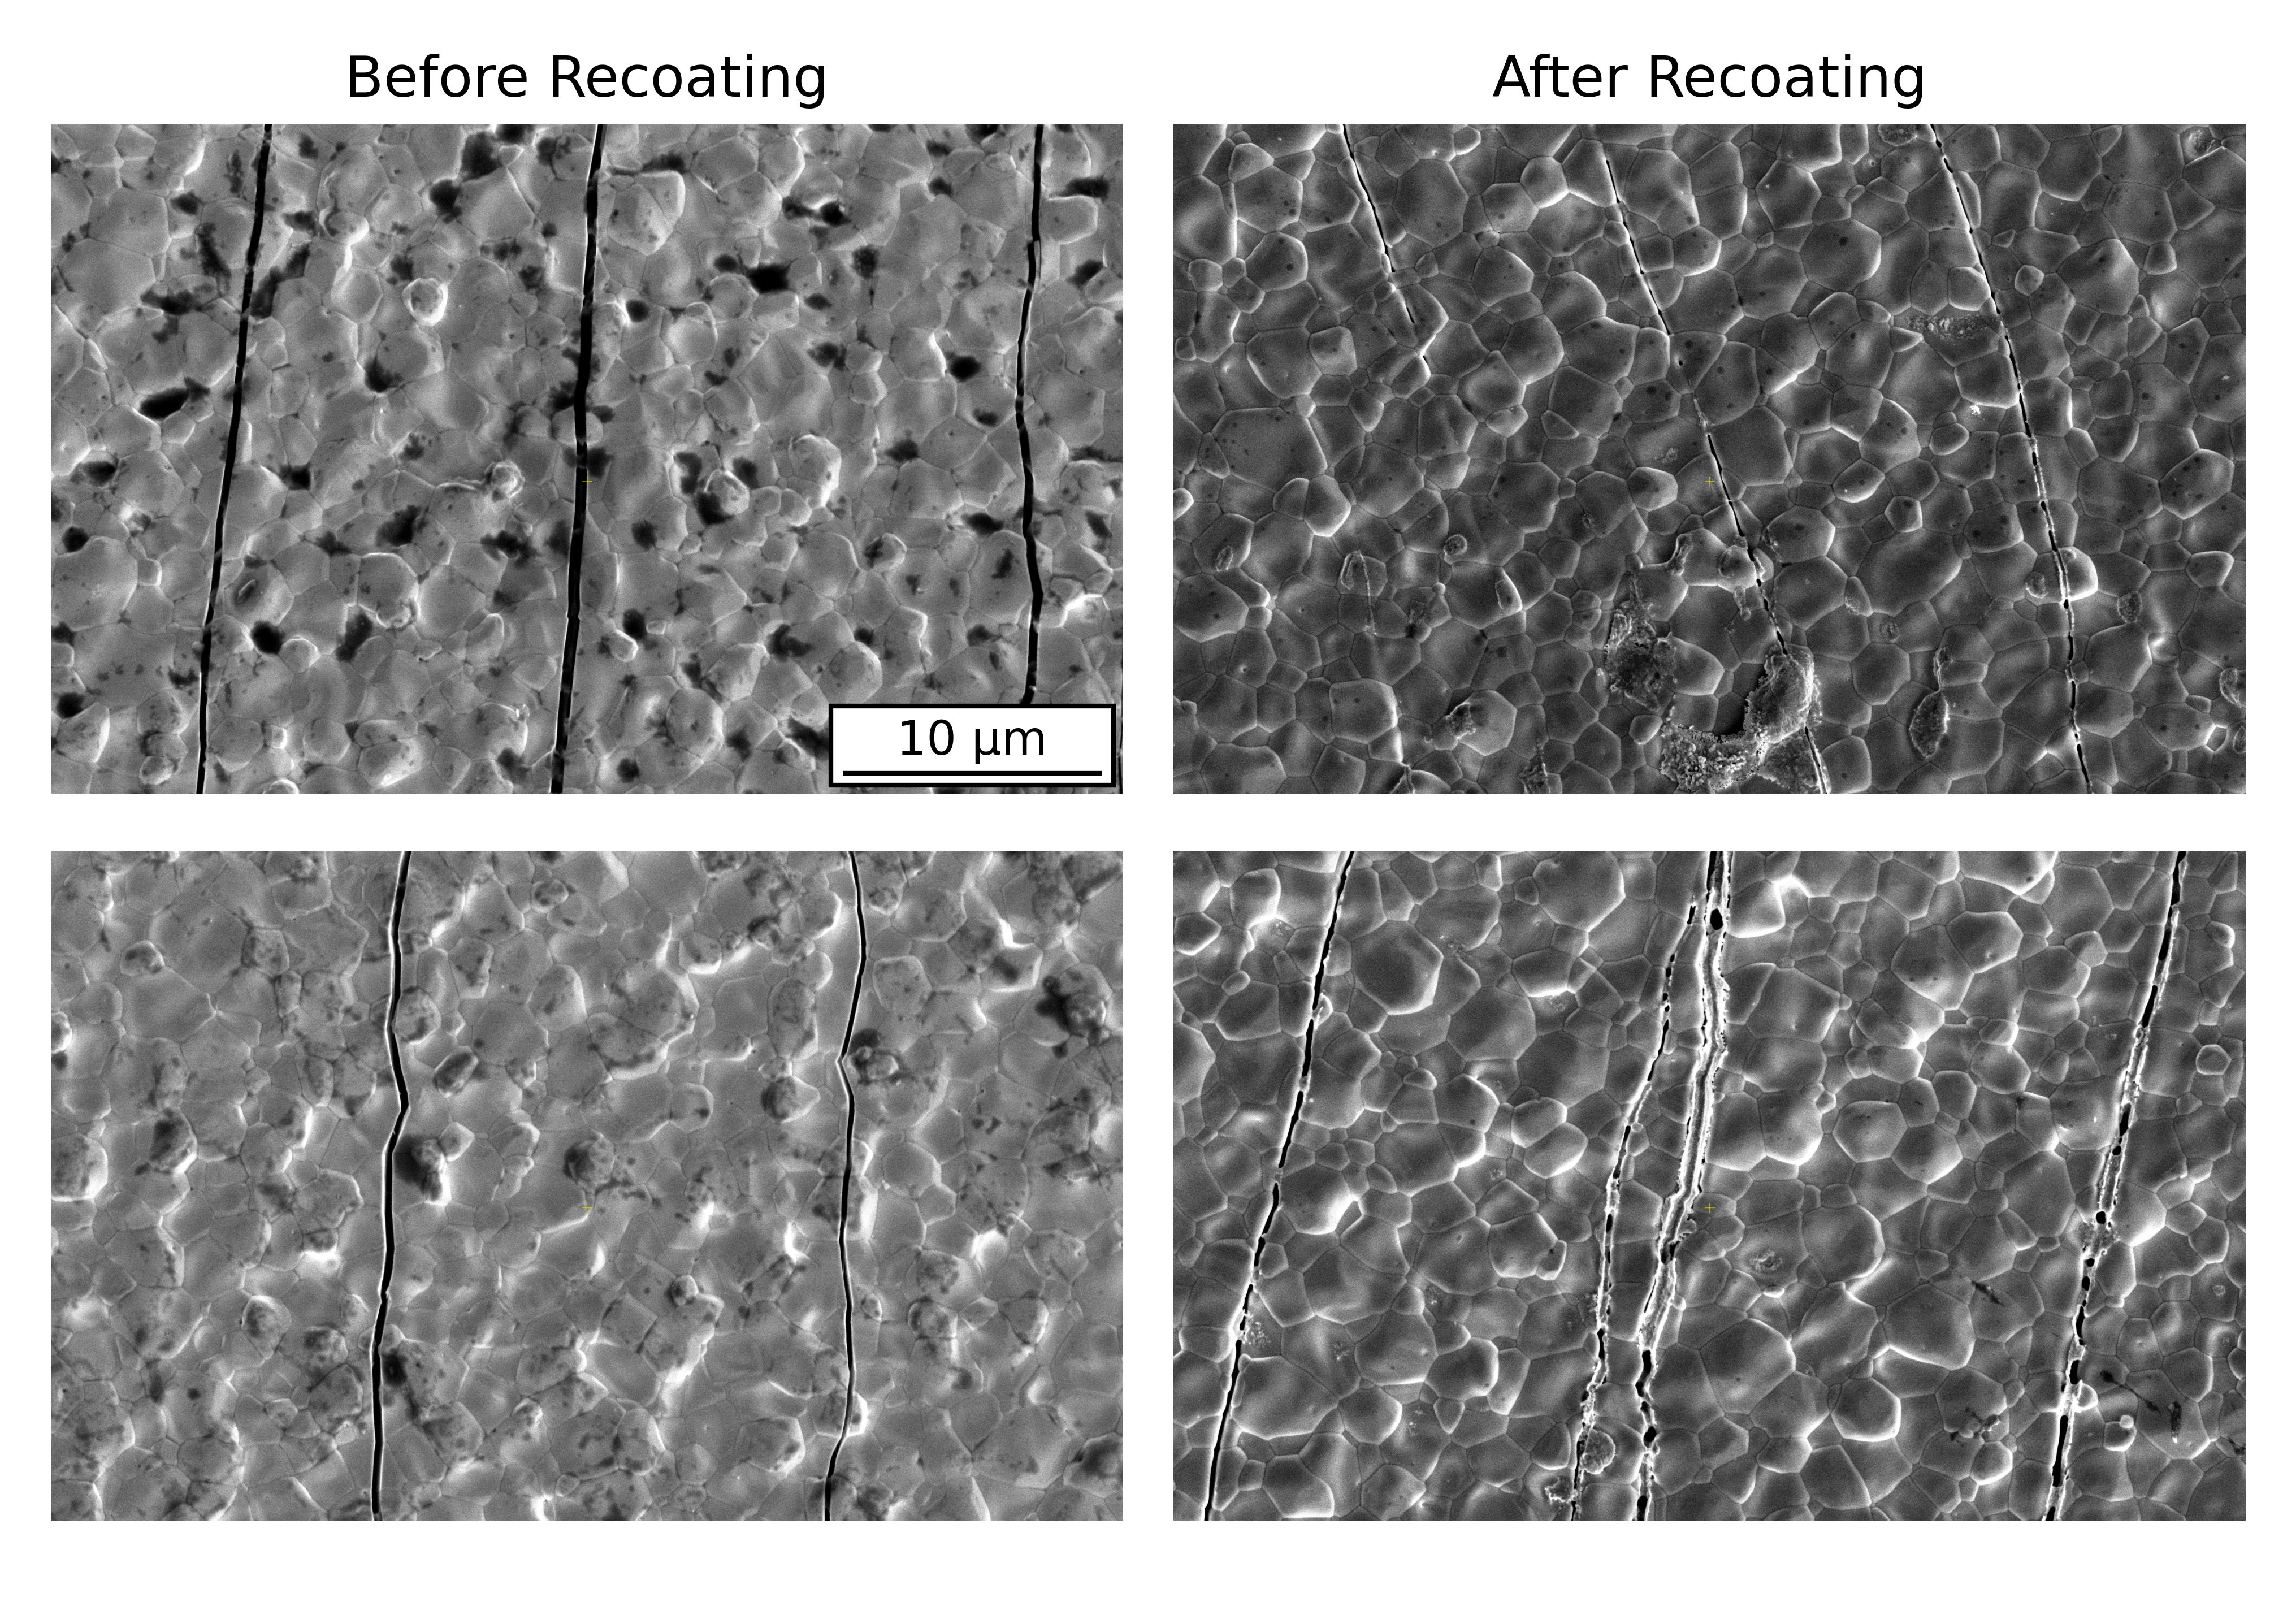
\includegraphics[]{./figures/SEM/SEM.png}
    \caption{This figure shows micrographs of elongated Nb\textsubscript{3}Sn coated wires. The left side shows the samples before treatment with recoating and the right side shows the samples after recoating. After the recoating treatment the cracks appear to be partially filled with new Nb\textsubscript{3}Sn.}
    \label{fig:SEM}
\end{figure}

\begin{figure}
    
    \includegraphics[]{./figures/EDS/EDS.png}
    \caption{The cross section of the film cracks is imaged using FIB/SEM before and after recoating. The Sn content of the cracks is measured qualitatively using Energy dispersive X-ray Spectroscopy (EDS). We find that there is new Nb\textsubscript{3}Sn material both in the crack and in the substrate at the base of the crack. There is no evidence of Sn rich phases in the crack.}
    \label{fig:EDS}
\end{figure}


\section*{Discussion}
\label{sec:Discussion}

Recoating a damaged Nb\textsubscript{3}Sn cavity can have a major impact on its performance. The recoating process was able to mostly recover both the maximum accelerating gradient and quality factor of the cavity. The degradation in quality factor seen at \qty{2}{\kelvin} at high fields seen in figure \ref{fig:VTS}, C is caused by a quench at \qty{16}{\mega\volt\per\meter} resulting in trapped flux. However, the cavity was able to reach a higher gradient of \qty{19}{\mega\volt\per\meter} after the initial quench. This is close to the \qty{24}{\mega\volt\per\meter} maximum field of the cavity before the degradation occured. It is possible that the cavity may recover more of its performance by using a longer recoating or other surface treatments such as mechanical polishing\cite{viklund2024improving}. 

The healing mechanism of the recoating is heretofor unknown. From our observations it appears that the healing occurs via two different processes, the creation of new Nb\textsubscript{3}Sn within the crack and the creation of Nb\textsubscript{3}Sn at the exposed Nb substrate at the base of the crack. This phenomenon has been studied in other thin film system and is known as self healing~\cite{Sloof2007}. Here we propose two mechanisms to explain the self healing observed in our experiments. 

The first mechanism for self healing is creation of newly formed Nb\textsubscript{3}Sn within the crack. When a cavity is exposed to Sn, a thin layer of liquid Sn coats the surface which thereby fills the cracks. Nb\textsubscript{3}Sn is then formed in the cracks by diffusion of Nb from the old Nb\textsubscript{3}Sn into the liquid Sn creating new Nb\textsubscript{3}Sn. The diffusion rate of Nb is relatively slow compared to the diffusion of Sn through the grain boundaries during normal film growth, however if the cracks are small, less than a few \qty{100}{nm}, Nb may have sufficient time to diffuse into the crack. The diffusion of Nb into the crack may be aided by dissolution of Nb\textsubscript{3}Sn into the liquid Sn layer above \qty{910}{\celsius} which would greatly boost the diffusion rate. Since Nb is diffusing from the Nb\textsubscript{3}Sn film into the crack, there is the possibility of creating non-superconducting Sn rich Nb-Sn phases such as Nb\textsubscript{6}Sn\textsubscript{5} and NbSn\textsubscript{2}. However, we see no evidence of these phases on the length scales measurable using EDS. Further analysis is required using higher resolution techniques such as transmission electron microscopy (TEM-EDS) to verify the stoichiometry of the newly created Nb\textsubscript{3}Sn material.

The second mechanism involves the diffusion of Sn into the Nb substrate through the crack. Since the crack penetrates the Nb\textsubscript{3}Sn film, the liquid Sn layer can come into contact with the crack and react with the Nb substrate creating a region of new Nb\textsubscript{3}Sn. This new region acts as a bridge for electrical currents to flow through the film and prevents current from flowing through the Nb substrate, which has a higher resistivity than does Nb\textsubscript{3}Sn. 


\section{Conclusion}
\label{sec:Conclusion}

Using a low temperature (\qty{1000}{\degreeCelsius}), short duration (\qty{1}{\hour}) Sn recoating process, we are able to heal a degraded Nb\textsubscript{3}Sn cavity that suffered damage during transportation. The recoating process improved the maximum gradient of the cavity from \qty{8}{\mega\volt\per\meter} to \qty{19}{\mega\volt\per\meter}, which is close to the initial performance of the cavity of \qty{24}{\mega\volt\per\meter}. Temperature mapping measurements of the cavity demonstrate that a single hot spot on the equator of the cavity was responsible for the performance degradation. After the recoating process this defect becomes healed leading to less heating and a higher maximum electric field gradient. Ultimately, the performance is limited by a second hot spot.

This discovery provides a new approach which applies to similarly degraded SRF cavities to recover their performances. This approach saves time and money which would otherwise be spent removing the Nb\textsubscript{3}Sn coating and then applying a new coating. This self healing process makes Nb\textsubscript{3}Sn cavities more viable for real-world accelerator applications by reducing their manufacturing costs.
